\documentclass{beamer}
\usepackage{hyperref}
\title{DNS message checksums}
\subtitle{\texttt{draft-muks-dnsop-dns-message-checksums-01}}
\author{Mukund Sivaraman}
\institute{Internet Systems Consortium}
\date{}

\begin{document}

\frame{\titlepage}

\section{Intro}
\frame
{
  \frametitle{IP layer fragmentation}

  \begin{itemize}
  \item IP layer PDUs (``packets'') can get fragmented --- broken into
    multiple pieces during transmission --- because they don't fit in
    the MTU somewhere on the path
  \item More IP fragments mean more opportunity for an off-path attacker
    to succeed in poisoning a reply by injecting spoofed fragments into
    a network
  \item Shopping list of problems in \textsl{``Fragmentation Considered
    Poisonous''} by Amir~Herzberg and Haya~Shulman

    % TBD Something about IP fragmentation induced by spoofing ICMP
    % destination unreachable (4 $\Rightarrow$ ``DF=1 but fragmentation
    % is required'') messages; Linux seems to apply discovered PMTU from
    % TCP, to UDP traffic by default (it is possible to disable it)

  \end{itemize}
}

\frame
{
  \frametitle{DNS message poisoning}

  \begin{itemize}
  \item UDP checksum is trivially defeated and is insufficient to
    protect against malicious modifications of datagrams
  \item RFC5452 anti-Kaminsky measures (random source port, random
    message ID) cannot be used in detecting message modification
    (poisoning); they can only be used in detecting spoofing at the
    whole-packet level
  \item DNS cookies similarly cannot be used in detecting message
    modification, except detecting spoofing at the whole-packet level
  \end{itemize}
}

\frame
{
  \frametitle{Other attacks with IP layer fragmentation}

  \begin{itemize}
  \item Response blocking --- attacker spoofs bogus fragments causing
    assembled UDP datagram to fail UDP checksum verification
  \item Nameserver blocking --- attacker repeatedly blocks responses
    from a nameserver, and resolver blacklists it denying itself access
    to the nameserver for all the zones it serves
  \item Nameserver pinning --- attacker causes resolver to repeatedly
    block nameservers for a zone, making the resolver limit itself to a
    nameserver of the attacker's choosing
  \item The general problem is that the IP layer is vulnerable as
    fragment assembly is controlled here. Higher layers may drop
    assembled packets from incorrect fragments and it's not possible to
    control fragment assembly from the higher layers, allowing
    unstoppable disruption to UDP while IP fragmentation is occurring.
  \item It is worth discussing making better use of \texttt{DF=1} and
    switch to application level fragmentation for larger responses (see
    DNS message fragments draft) where we control assembly.
  \end{itemize}
}

\frame
{
  \frametitle{On-path and off-path attackers}

  \begin{itemize}
    \item Off-path attackers are only able to attempt poisoning and
      disrupting some traffic
      \begin{itemize}
      \item Unable to snoop on packets (no loss of privacy)
      \item Able to inject forged packets (poisoning)
      \item Unable to filter packets (no loss of service)
      \item Effects: Poisoning of data, some control (protocol
        information), cause havoc with IP fragments
      \item Solution: Strong checks and application level fragmentation
        with \texttt{DF=1} are reasonable protection measures
      \end{itemize}
    \item On-path attackers may be able to observe, poison and disrupt
      all traffic
      \begin{itemize}
      \item May be able to snoop on packets (loss of privacy)
      \item May be able to inject forged packets (poisoning)
      \item May be able to filter packets (loss of service)
      \item Effects: MITM attacks, TCP RSTs, packet drops, total chaos
      \item Solutions: Cryptographic signatures (including for control
        --- e.g., TLS cannot stop TCP reset injection), encryption; even
        then nothing can be done to prevent total loss of service
      \end{itemize}
  \end{itemize}
}

\frame
{
  \frametitle{``Just use DNSSEC!''}

  \begin{itemize}
  \item RRSIGs can be used to validate the contents of RRsets
  \item DNSSEC does not protect contents of messages that do not have
    RRSIGs, such as NS records and glue at a delegation point in a
    referral, and EDNS0 options
  \item DNSSEC cannot be used to validate {\em what} RRs a server sent
    to a client, only the contents of RRs. A stupid example:
    \begin{itemize}
    \item Consider a HTTP service `files.example.com' with address
      192.0.2.1 for users in Japan and address 198.51.100.1 for users in
      China, which are only accessible from those countries respectively
      --- there is no route to these addresses from outside the
      respective country
    \item NS serves A~192.0.2.1 to Japan, A~198.51.100.1 to China
      using views. The zones are signed with the same KSK and ZSK.
    \item Attacker who's able to spoof traffic in China uses shell
      account in Japan to grab DNS message for Japan and poisons
      resolver in China with Japan's address record with its correct
      RRSIG.
    \item User in China is unable to access `files.example.com' using an
      address from \texttt{AD=1} reply because there's no route.
    \end{itemize}
  \end{itemize}
}

\frame
{
  \frametitle{``Just use TCP!''}

  \begin{itemize}
  \item UDP has annoying problems allowing poisoning, amplification
    attacks, etc. In DNS, they are mostly known and addressed.
  \item DNS over TCP doubles roundtrips compared to UDP. Name resolution
    involves iteration including indirection (out-of-bailiwick NS
    referral) during lookup. As DNS lookup is at the head of any list of
    network operations, it increases the turnaround time of every item
    on the list when resolution is required. This is very conspicuous in
    parts of the world with large RTTs to the majority of nameservers
    for domains of medium-to-high popularity and must not be ignored.
  \item Truncating UDP on purpose to force TCP is worse. It triples
    RTT (1 for UDP attempt, +2 until TCP first data).
  \item See \texttt{5966bis} for commentary on performance of DNS over
    TCP vs. UDP.
  \end{itemize}
}

\section{Design}

\frame
{
  \frametitle{The EDNS CHECKSUM option proposal}

  \begin{itemize}
  \item This option aims to protect against \textbf{off-path message
    poisoning attacks on DNS messages} including those performed by
    taking advantage of IP~fragmentation.
  \item CHECKSUM tries to protect UDP DNS traffic in its existing form
    from modifications.
  \end{itemize}
}

\frame
{
  \frametitle{DNS message with CHECKSUM --- \texttt{QR=0}}

  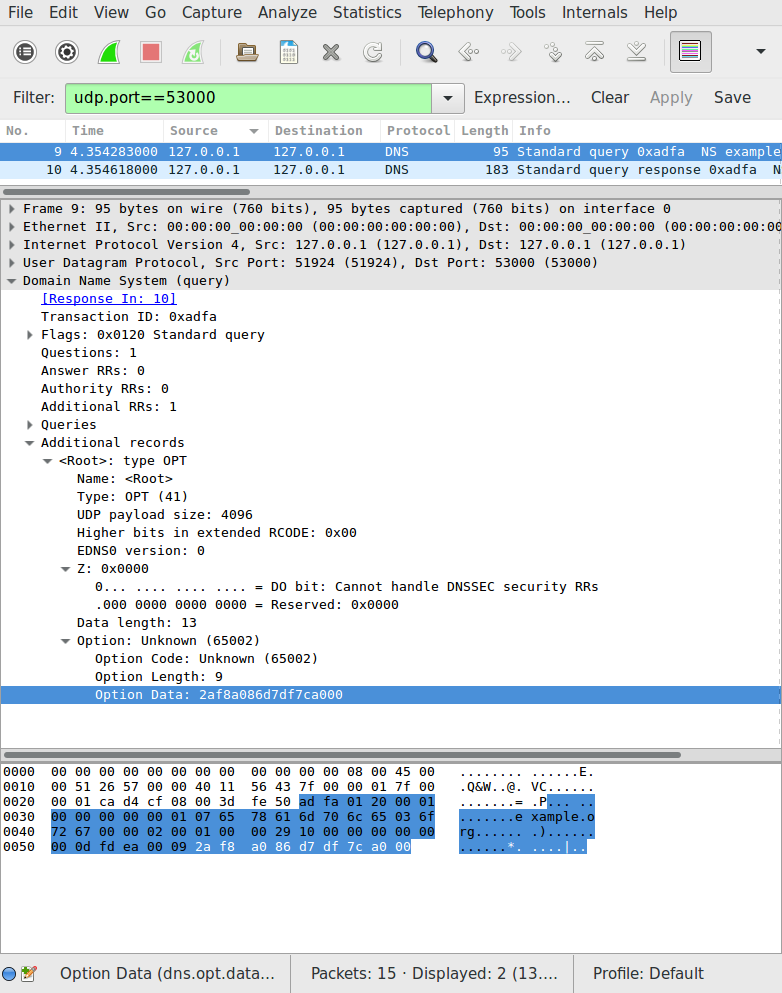
\includegraphics[height=20em]{qr0.png}
}

\frame
{
  \frametitle{DNS message with CHECKSUM --- \texttt{QR=1}}

  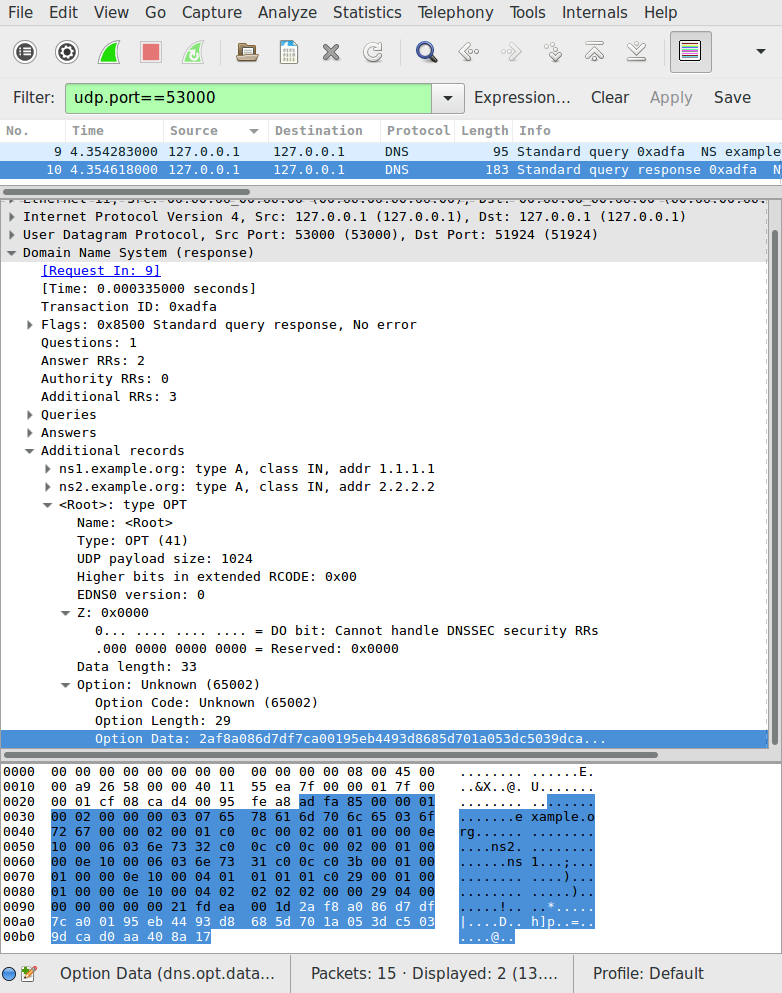
\includegraphics[height=20em]{qr1.png}
}

\frame
{
  \frametitle{Security considerations}

  \begin{itemize}
  \item CHECKSUM cannot protect against UDP checksum validation failures
    due to spoofed IP fragments, causing response blocking, NS blocking
    and NS pinning. DNS message fragments can be used in addressing
    these problems.
  \item On-path message poisoning is better handled by DPRIVE; would
    require significantly different operation and possible protocol
    changes.
  \end{itemize}
}

\frame
{
  \frametitle{Open issues}

  \begin{itemize}
  \item TBD.
  \end{itemize}
}

\section{Conclusion}
\frame
{
  \frametitle{\texttt{100 END}}

  Thanks for watching.

  \vskip 2em

  A BIND implementation is in the \texttt{dns-message-checksums} branch
  at: \url{https://github.com/muks/bind9/}
}

\end{document}
